
\section{Team PML 30 --${X}$} 
Team PML 30 -- ${X}$ was assembled in September 2014 in the Russian city of St. Petersburg from 3 novices and 2 participants with experience. Tasks and roles were distributed among the participants, and we established safety rules. In the first place the team put spreading principles of gracious professionalism to others. All decisions were made collectively inside team with discussion to find the most optimal solutions. 
During the year we took part in many events and everywhere we have tried to attract attention to our team and encourage people to take part in FTC. Also we pursued and distributed the principles of honorable professionalism. Talking to the press, we hoped to attract more attention to our team and to the competition in general, as well as attracting sponsors. The latter was important because of the need for funds - purchasing materials and equipment costs a lot.
The team took part in the three qualifying competitions and in the regional finals. In all of them we made new contacts, shared experience and provided mutual assistance to other teams. In the first qualifying rounds in Sochi we met Stuy Fission 310 from USA and maintain contact with them to this day. On regional finals, we met with a team from Romania, Auto Vortex, and keep in touch with them through Facebook. Also, there is an active group chat with a large number of Russian teams. You can find the team page in Facebook at the address https://www.facebook.com/pages/FTC-team-PML30-PHI.
To increase the efficiency of our team work we used the version control system GitHub, which allows the entire team to work simultaneously on a single projects without losing files and providing easy way to resolve roblems. Also for writing technical books we been used professional typesetting system LaTeX.
\begin{figure}[H]
	\center{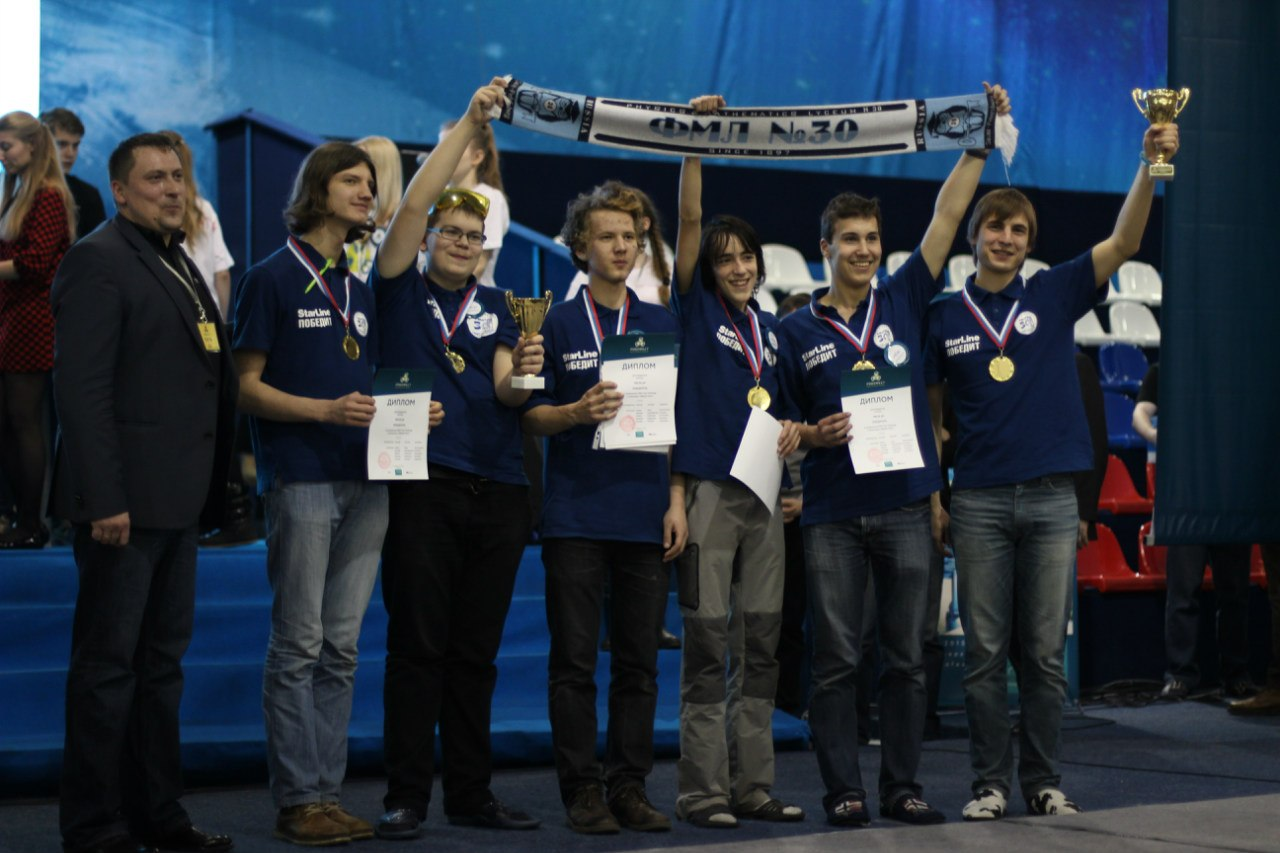
\includegraphics[scale=0.2]{1Introduction/2Our_team/images/09}}\\
\end{figure}[H]
\fillpage

\subsubsection{Instructors}

\begin{figure}[H]
	
	\begin{minipage}[h]{0.47\linewidth}
		Luzin Dmitry\\
		\emph{Head of Robotics Department in Phys-Math Lyceum 30, Saint-Peterburg, Russia. Main coach of FTC team.\\}
		\emph{Information: 25 years old, in robotics 5 years, in FTC 3 years.}
	\end{minipage}
	\hfill
	\begin{minipage}{0.47\linewidth}
		\center{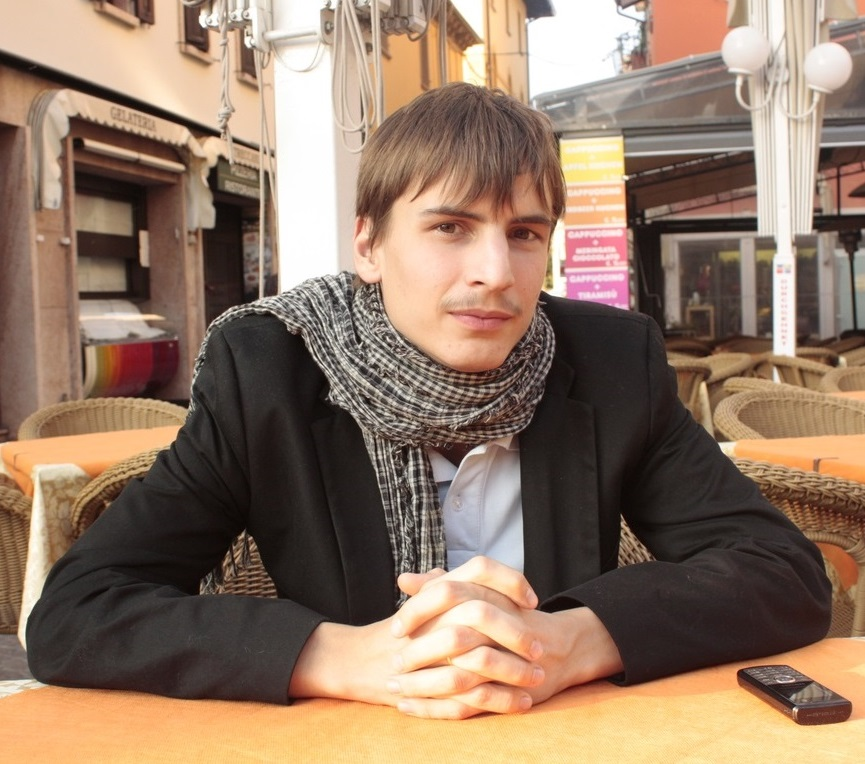
\includegraphics[scale=0.3]{1Introduction/2Our_team/images/07}}\\
	\end{minipage}
	\vfill
	\begin{minipage}[h]{0.47\linewidth}
		\center{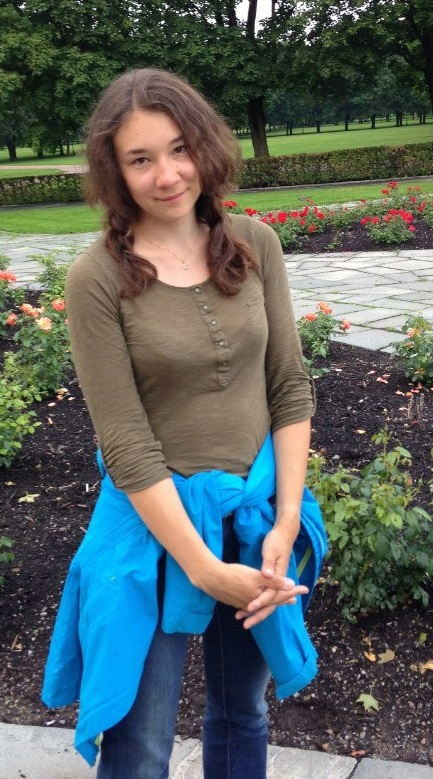
\includegraphics[scale=0.35]{1Introduction/2Our_team/images/08}}\\
	\end{minipage}
	\hfill
	\begin{minipage}{0.47\linewidth}
		Luzina Ekaterina \\
		\emph{Professor of Robotics Department in Phys-Math Lyceum 30, Saint-Peterburg, Russia. Tutor of FTC team. \\}
		\emph{Information: 25 years old, in robotics 5 years, in FTC 3 years.}
	\end{minipage}
\end{figure}

\begin{figure}[H]
	\begin{minipage}[h]{0.47\linewidth}
		\center{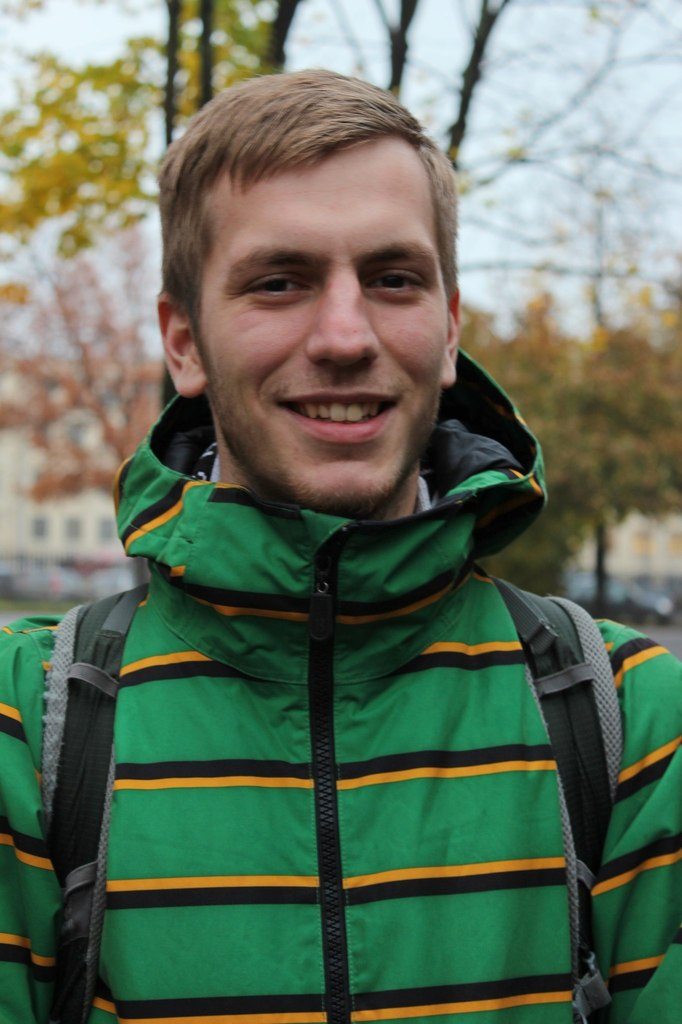
\includegraphics[scale=0.25]{1Introduction/2Our_team/images/05}}\\
	\end{minipage}
	\hfill
	\begin{minipage}{0.47\linewidth}
		Fedotov Anton \\ 
		\emph{Professor of Robotics Department in Phys-Math Lyceum 30, Saint-Peterburg, Russia. Tutor of FTC team. \\}
		\emph{Information: 22 years old, in robotics 4 years, in FTC 3 years.}
	\end{minipage}	
	\vfill 
\end{figure}

\begin{figure}[H]
	\begin{minipage}{0.47\linewidth}
		Krylov Georgii \\ 
		\emph{Professor of Robotics Department in Phys-Math Lyceum 30, Saint-Peterburg, Russia. Tutor of FTC team. \\}
		\emph{Information: 18 years old, in robotics 4 years, in FTC 4 years.}
	\end{minipage}	
	\hfill
	\begin{minipage}[h]{0.47\linewidth}
		\center{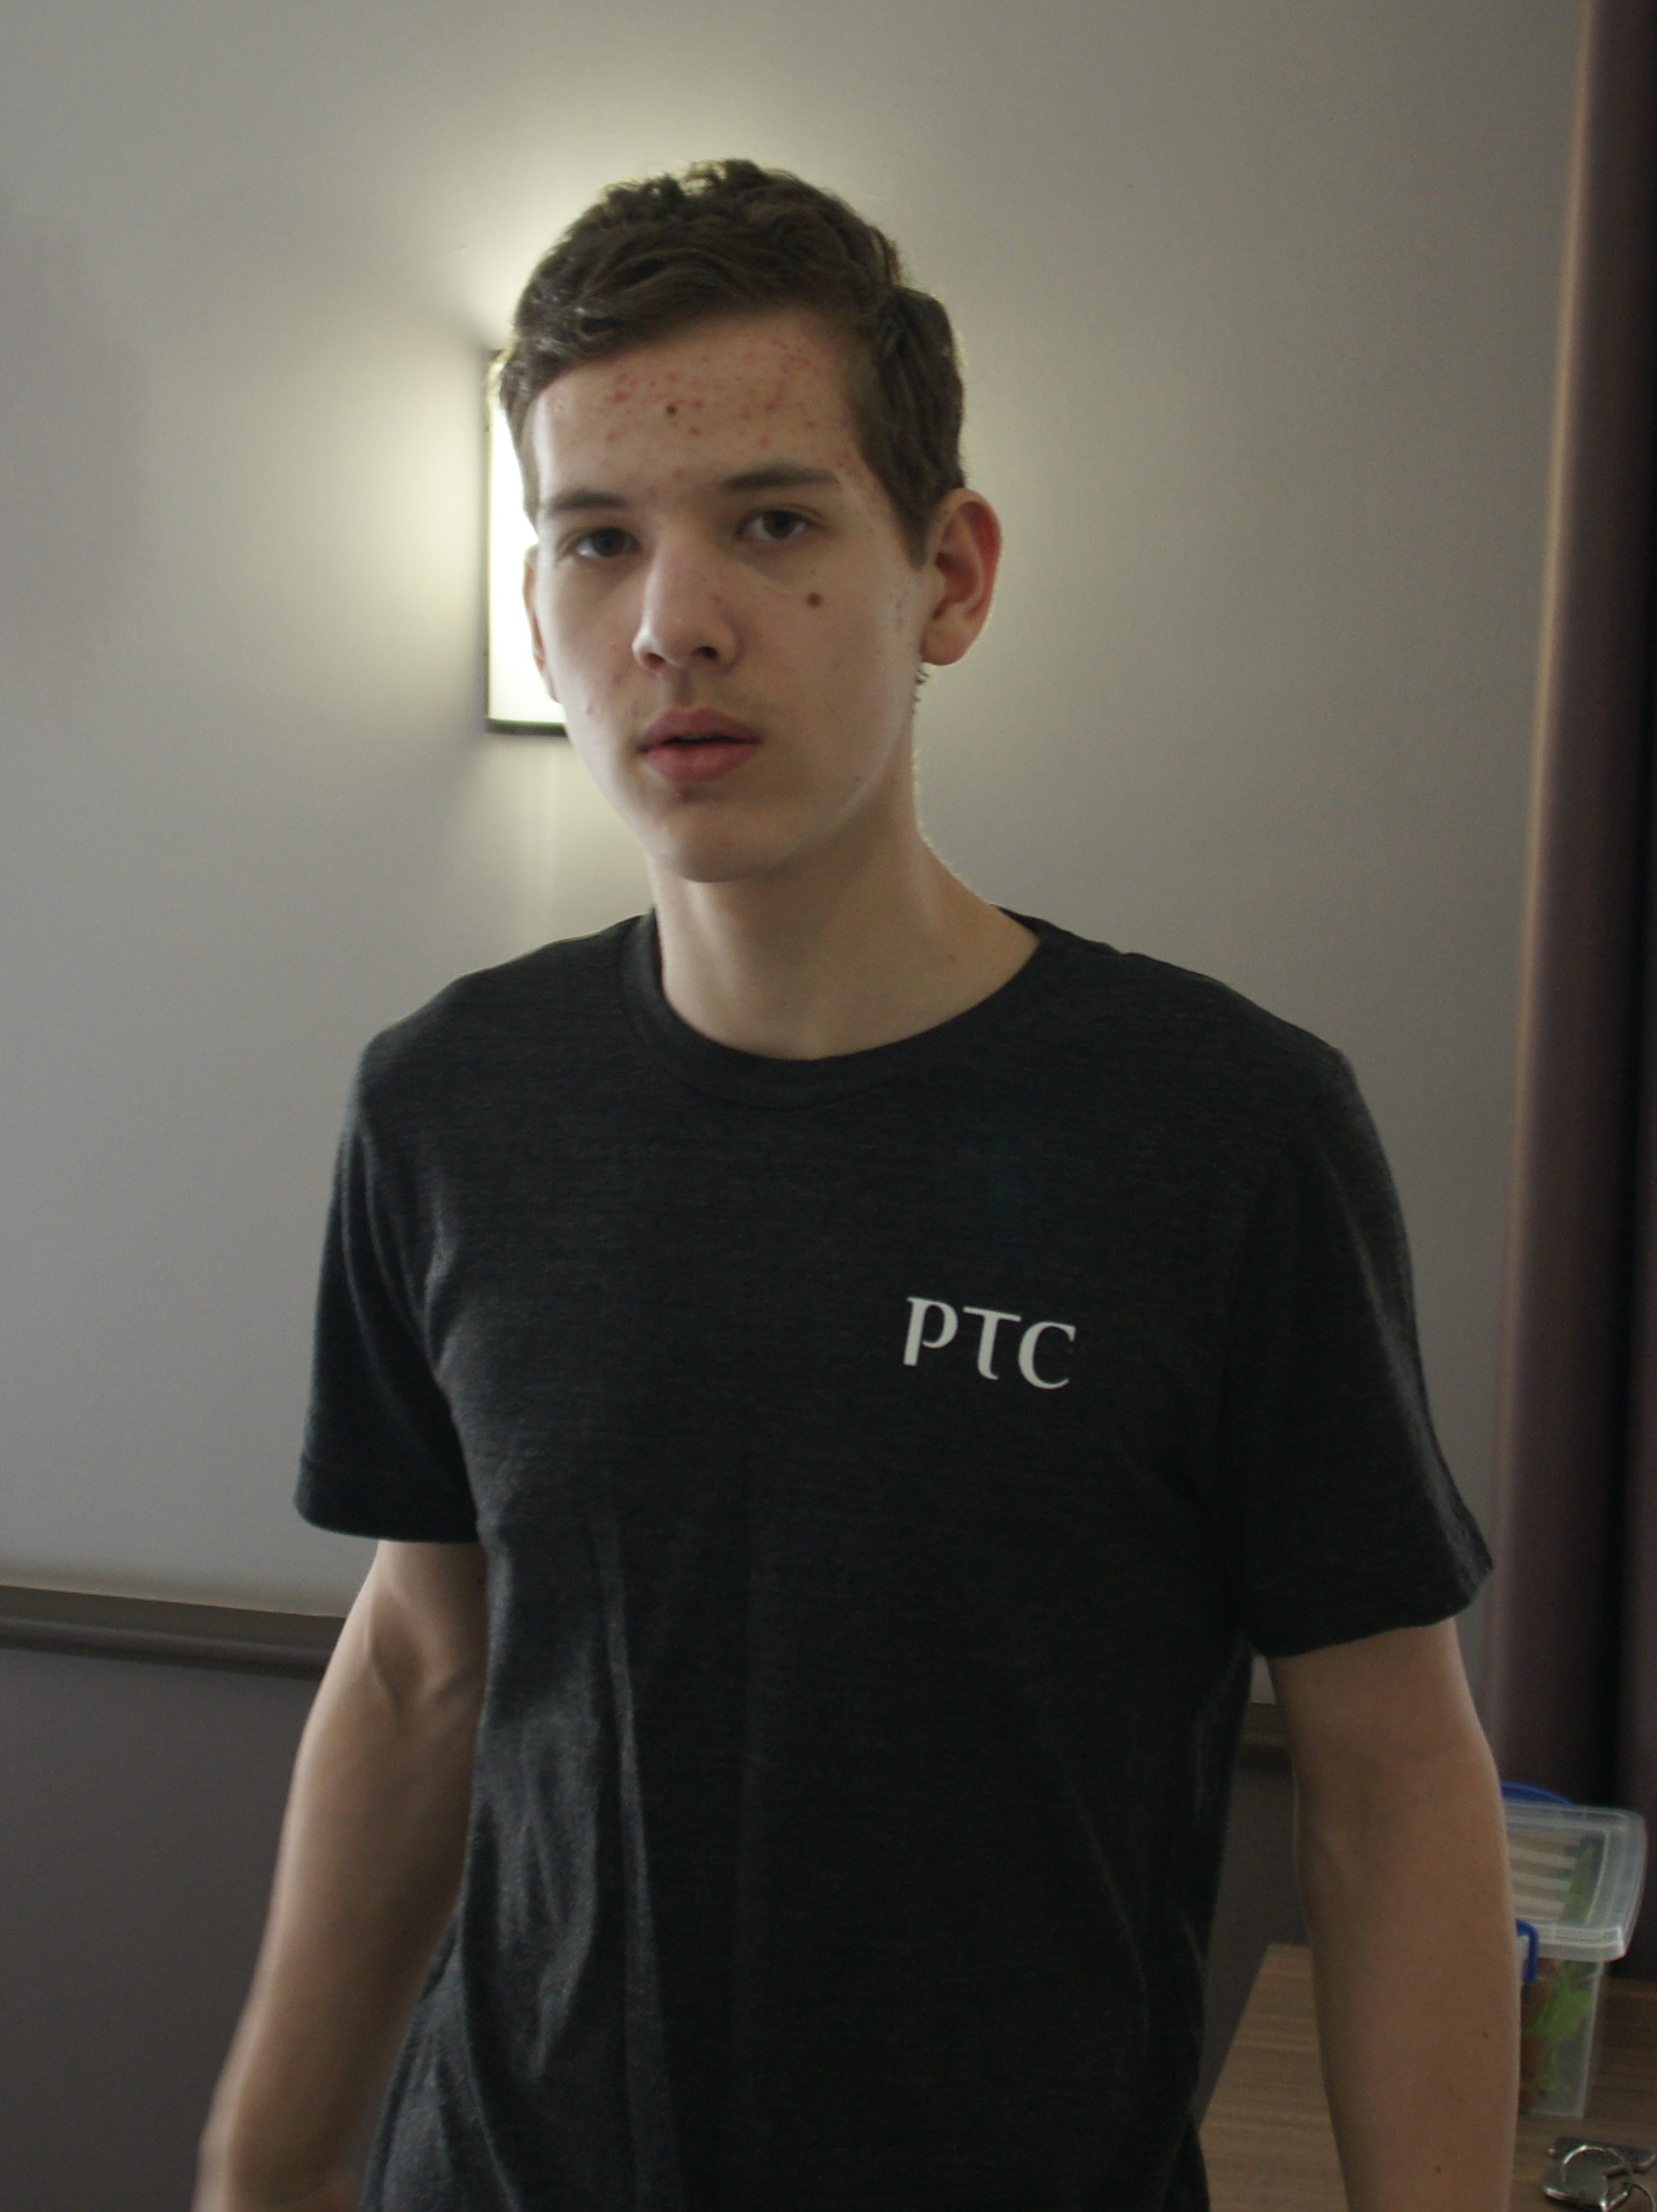
\includegraphics[scale=0.11]{1Introduction/2Our_team/images/06}}\\
	\end{minipage}
	\vfill 
\end{figure}

\fillpage

\subsubsection{Team members}
\begin{figure}[H]
	\begin{minipage}[h]{0.47\linewidth}
		\center{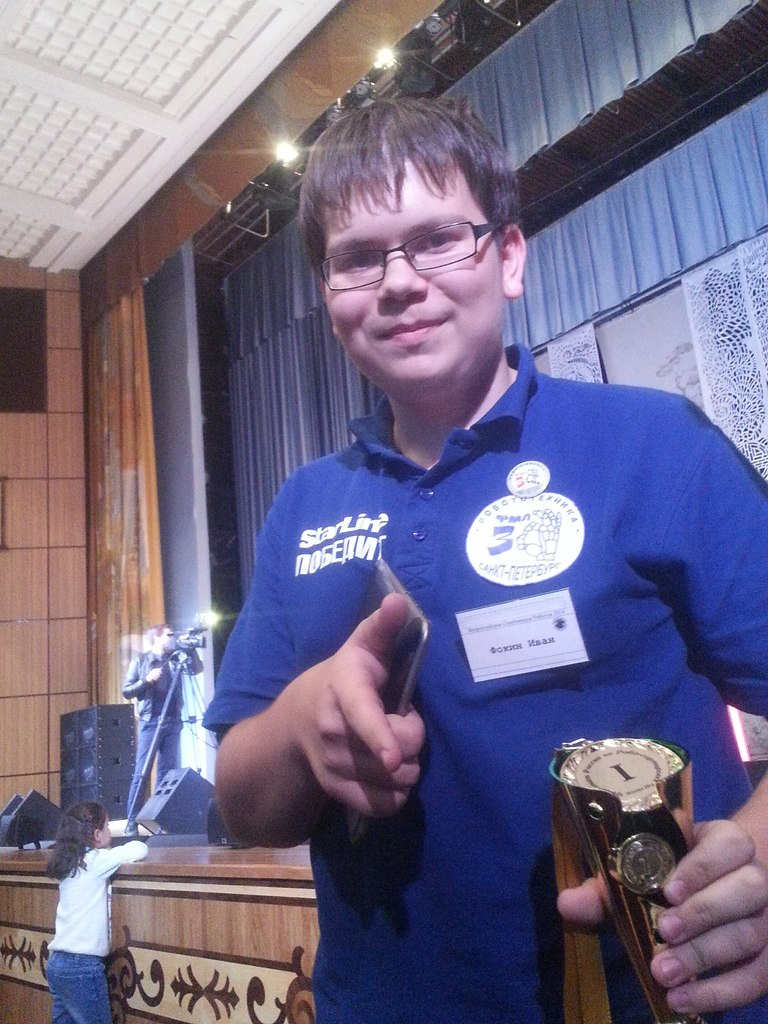
\includegraphics[scale=0.5]{1Introduction/2Our_team/images/01}}		
	\end{minipage}
	\hfill
	\begin{minipage}[h]{0.47\linewidth}
		Aleksandr Iliasov \\
		\emph{Role in team: reserve operator-1, responsible for the safety precaution, responsible for the bucket.\\}
		\emph{Information: 16 years old, in robotics 3 years, in FTC 2 years. \\}
		\emph{Why I chose FTC: ""}		
	\end{minipage}
	\vfill 
	\begin{minipage}[h]{0.47\linewidth}
		Anton Ponikarovskiy\\
		\emph{Role in team: captain, communication with other teams and community, reserve operator-2, responsible for the elevator. \\  }
		\emph{Information: 17 years old, in robotics 3 years, in FTC 2 years. \\}
		\emph{Why I chose FTC: ""}					
	\end{minipage}
	\hfill
	\begin{minipage}[h]{0.47\linewidth}
		\center{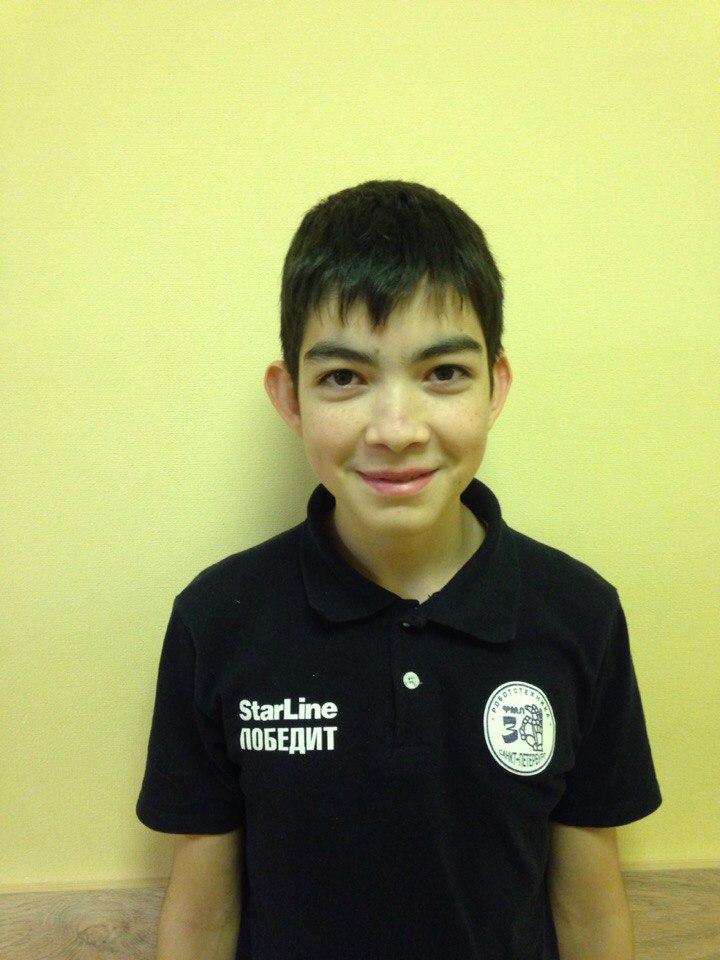
\includegraphics[scale=0.25]{1Introduction/2Our_team/images/02}}\\
	\end{minipage}
	\vfill
	\begin{minipage}{0.47\linewidth}
		\center{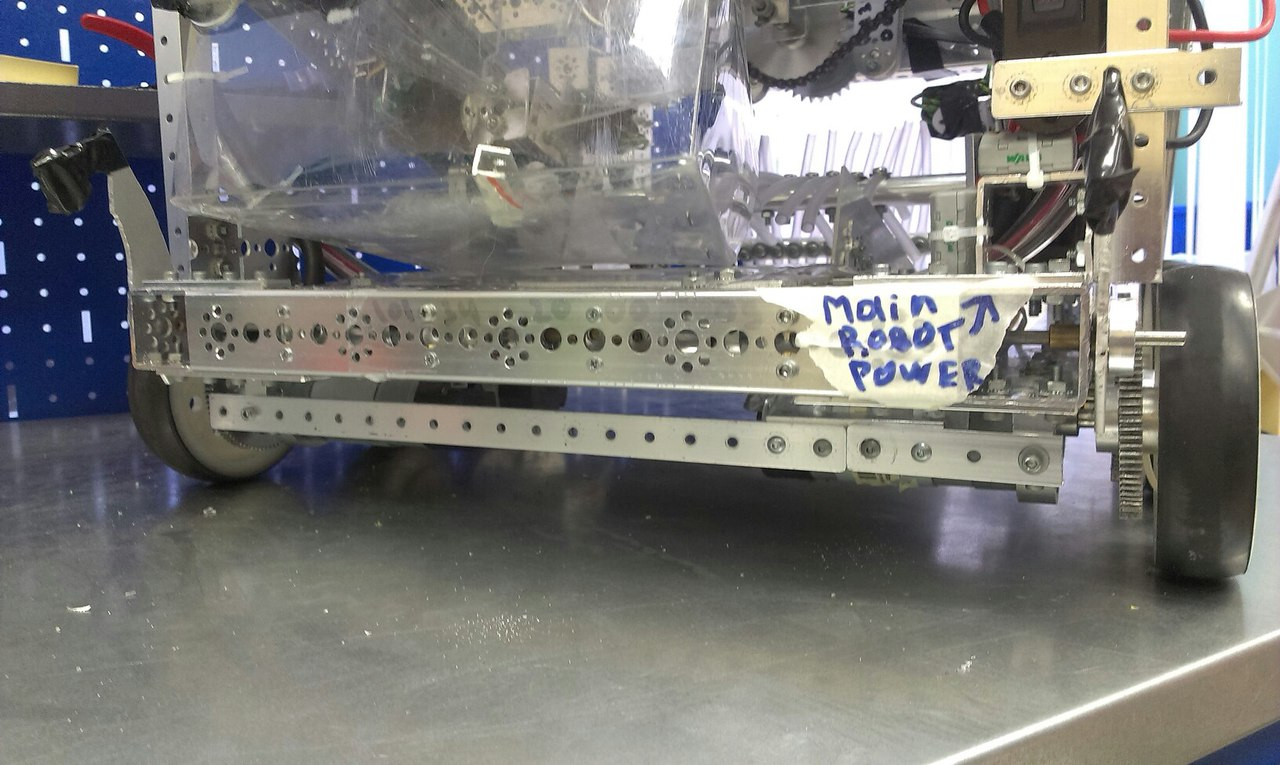
\includegraphics[scale=0.22]{1Introduction/2Our_team/images/03}}\\
	\end{minipage}
	\hfill
	\begin{minipage}{0.47\linewidth}
		Gordei Kravtsov\\
		\emph{Role in team: operator-2, responsible for the writing of technical book, responsible for the wheel base. \\}
		\emph{Information: 17 years old, in robotics 2 years, in FTC 1 year.\\} 
		\emph{Why I chose FTC: ""}				
	\end{minipage}
\end{figure}

\begin{figure}[H]
	\begin{minipage}{0.47\linewidth}
		Andrei Nemov\\
		\emph{Role in team: operator-1, responsible for the safety precaution, responsible for the writing of technical book, responsible for the debris collecting system. \\}
		\emph{Information: 16 years old, in robotics 2 years, in FTC 1 year. \\}
		\emph{Why I chose FTC: "When I first I attended the event FTC saw hefty metal robots, with enthusiasm and without hesitation decided that I would like to do this."}			
	\end{minipage}
	\hfill
	\begin{minipage}{0.47\linewidth}
		\center{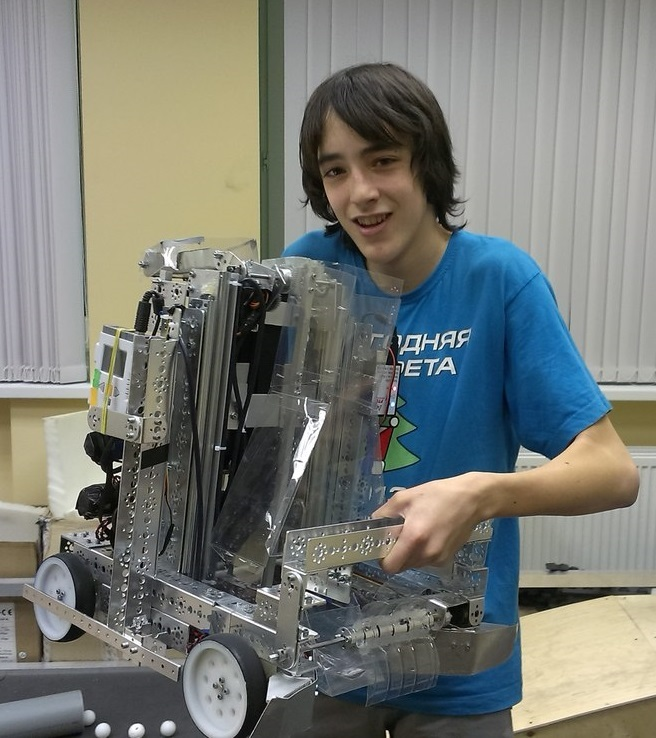
\includegraphics[scale=0.25]{1Introduction/2Our_team/images/04}}\\
	\end{minipage}	
\end{figure}
\vfill	
\begin{minipage}{0.47\linewidth}
	\center{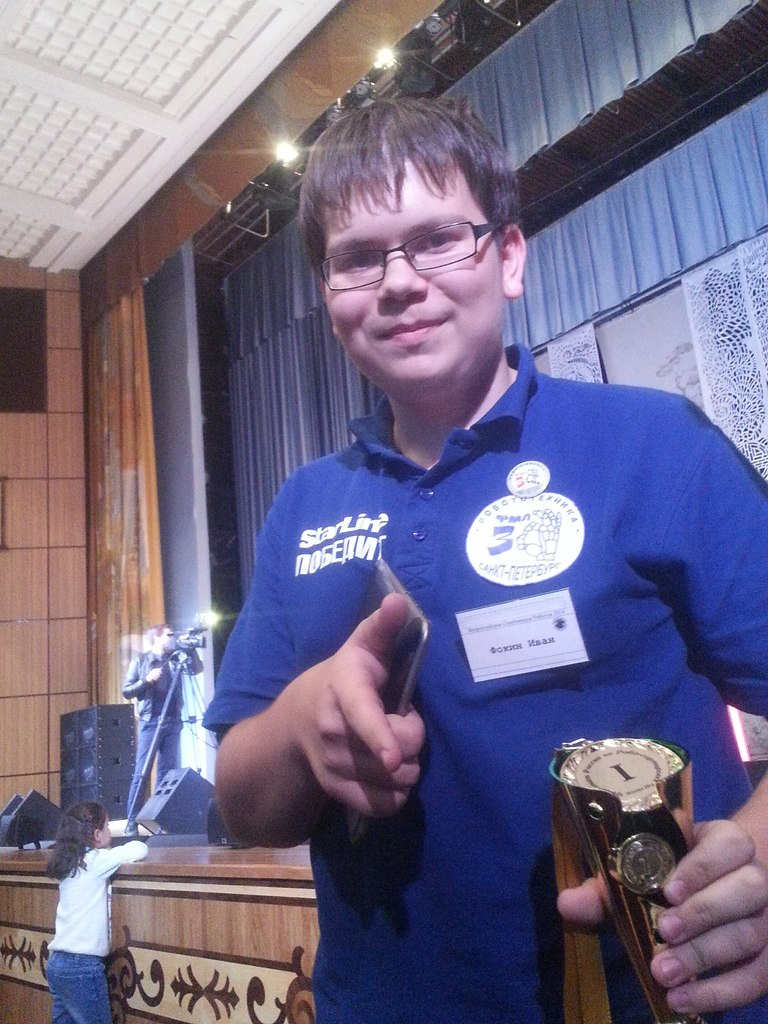
\includegraphics[scale=0.2]{1Introduction/2Our_team/images/01}}			
\end{minipage}
\hfill
\begin{minipage}{0.47\linewidth}
	Timur Babadjanov\\
	\emph{Role in team: development strategy in the game, responsible for mechanisms for scoring climbers.\\ }
	\emph{Information: 16 years old, in robotics 2 years, in FTC 1 year. \\ } 
	\emph{Why I chose FTC:""}		
\end{minipage}

\fillpage


